
\section{Consistency sans Coordination}
\label{sec:bcc-theory}

With a system model and formal goals in hand, we now address the
question: when does transaction processing require synchronous
coordination? The answer depends on the set of operations the database
may be expected to perform as well as the integrity constraints that
the database is required to maintain. Unsurprisingly, combinations
fall into both categories. Our contribution here is to formalize a
criterion that will answer this question for specific transactions and
invariants---while only reasoning about transaction logic and
invariants.

\subsection{\iconfluence: Criteria Defined}

To begin, we introduce a concept that will underly our main result:
invariant confluence (hereafter,
\iconfluence)~\cite{obs-confluence}. Applied in a transactional
context, the \iconfluence property informally ensures that divergent,
valid database states can be merged into a valid database state. That
is, if the effects of two valid series of transactions ($S_i$, $S_j$)
that operate independently on the same copy of valid database state
produce valid outputs ($I(S_i(D))$ and $I(S_j(D))$ hold), their
effects can safely be combined to produce a valid database state
($I(S_i(D) \sqcup S_j(D))$ holds). \iconfluence will form the formal
basis of a relationship between \cfreedom and an application.

We first define a valid sequence of transactions, representing the
result of applying a set of transactions to database state such that
each intermediate state is valid; this captures the process of
applying transactions to a single database state and transitively
maintaining validity:

\begin{definition}[Valid Sequence]
Given invariant $I$, transactions $T$, and database state $D$,
$S_i(D)$ is an $I$-valid sequence of transactions in $T$ if $S_i(D) =
t_{in}(\dots t_{i1}(D))$, $\{t_{i1}, \dots, t_{in}\} \in T$, and
$\forall k \in [1, n], t_{ik}(\dots t_{i1}(D))$ is $I$-valid.
\end{definition}

Using the concept of valid sequences, we can formalize the
\iconfluence property, which requires that valid sequences with a
common ancestor are also valid under merge:

\begin{definition}[\iconfluence]
Transactions $T$ are \iconfluent with respect to invariant $I$ if, for
all $I$-valid sequences $S_1(D_0)$, $S_2(D_0)$ of transactions in $T$,
$I(S_1(D_0) \sqcup S_2(D_0))$ is $I$-valid.
\end{definition}

Figure~\ref{fig:iconfluence} depicts an \iconfluent execution using
two valid sequences each starting from the initial database state
$D_0$. This execution model will be familiar to users of fork-join
programming models~\cite{hewitt-forkjoin} (e.g., version control
systems like Git and Subversion). \iconfluence allows users to ``check
out'' a known good copy of database state ($D$ such that $I(D)$ holds)
and perform a series of modifications ($S_i$) to the state in
isolation---as long as these modifications are ``safe'' ($I(S_i(D))$
is true). Under \iconfluent operations, any concurrent series of
modifications to database state can be safely ``merged'' to provide a
valid database state ($I(S_1(D) \cup S_2(D))$ is true). We require
that $I$-valid sequences of transactions have a common ancestor to
rule out the possibility of merging arbitrary states that could not
have arisen from transaction execution (e.g., even if no transaction
assigns ids, it may be invalid to merge two states that each have
unique but overlapping sets of ids).

\iconfluence holds for some combinations of invariants and
transactions but not others. For example, if $I=\{$\textit{no bank
  account has negative balance}$\}$, then $T=\{$\textit{increment user
  A's balance by 100, increment user A's balance by 50}$\}$ is
\iconfluent, as is $T\cup\{$\textit{audit the database and store the
  sum of user balances in the \textrm{audit} table}$\}$ but not
$T\cup\{$\textit{decrement user A's balance by 200}$\}$. For now, our
goal will be to use this property in the abstract, but we will provide
a full discussion of practical uses in Section~\ref{sec:bcc-practice}.

\begin{figure}
\begin{center}
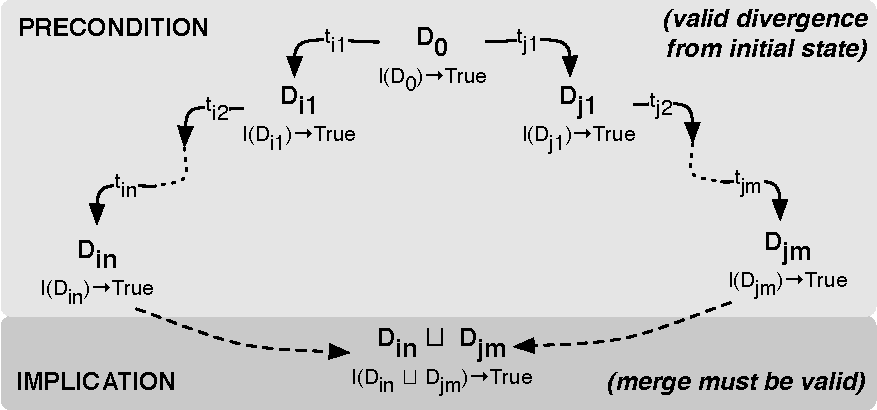
\includegraphics[width=\columnwidth]{figs/icommute.pdf}\vspace{-1em}
\end{center}
\caption{The \iconfluence property illustrated via a diamond
  diagram. If a set of transactions $T$ is \iconfluent, then all
  database states ($D_{in}$, $D_{jm}$) produced by $I$-valid sequences
  in $T$ starting from the initial database state ($D_0$) must be
  mergeable ($\sqcup$) into an $I$-valid database state.}
\label{fig:iconfluence}
\end{figure}

\subsection{\iconfluence and Coordination}

We can apply \iconfluence to our goals from Section~\ref{sec:model}:

\begin{theorem}
\label{theorem:necessary}
A globally $I$-valid system can execute transactions $T$ with
\cfreedom, transactional availability, convergence if and only if $T$
are \iconfluent with respect to $I$.
\end{theorem}

Theorem~\ref{theorem:necessary} establishes \iconfluence as a
necessary and sufficient condition for coordination-free
execution---the first such condition we are aware of. Effectively, we
have ``lifted'' the specification of semantics that are achievable
with scalability, availability, and low-latency to the level of
invariants and transactions. If \iconfluence holds, these goals are
attainable; if not, there is no possible implementation or execution
strategy that can guarantee these properties for the provided
invariants and transactions. That is, if \iconfluence does not hold,
there exists at least one execution of transactions on divergent
replicas that will violate the given invariants when replicas
converge. To prevent invalid states from occuring, at least one of the
transaction sequences will have to forego availability or \cfreedom,
or the system will have to forego convergence. This is a useful
result, and we will spend much of the remainder of the paper applying
it.

Before doing so, we first prove Theorem~\ref{theorem:necessary}. The
proof is based on both a proof by construction and classic
partitioning arguments~\cite{gilbert-cap}. Informally, if \iconfluence
holds, each replica can simply check each transaction's modifications
locally and replicas can simply merge independent modifications to
guarantee convergence to a valid state. For the converse, we construct
a scenario under which a replica cannot determine whether or not a
non-\iconfluent update should succeed without contacting another
replica, diverging forever, or compromising availability.

\begin{proof}
($\Leftarrow$) We begin with the simpler proof, which is by
  construction. Assume a set of transactions $T$ are \iconfluent with
  respect to an invariant $I$. Consider a system in which each replica
  executes the transactions it receives against a copy of its current
  state and checks whether or not the resulting state is $I$-valid. If
  the resulting state is $I$-valid, the replica commits the
  transaction. If not, the replica aborts the transaction. Replicas
  exchange copies of their local states and merge them. No individual
  replica will contain an invalid modification, and, because $T$ is
  \iconfluent under $I$, the merge of any two $I$-valid replica states
  as constructed above (i.e., valid sequences) is $I$-valid;
  therefore, the converged database state will be valid. Transactional
  availability, convergence, and global $I$-validity are all
  maintained via coordination-free execution.

($\Rightarrow$) Assume a system $M$ exists that can guarantee globally
  valid operation for a set of transactions $T$ with \cfreedom,
  transactional availability, and convergence, but $T$ is not
  $I$-confluent. Then there exists valid sequences $S_1,S_2$ in $T$
  such that $I(S_1(D_0)) \wedge I(S_2(D_0)) \rightarrow true$ but
  $I(S_1(D_0) \sqcup I(S_2(D_0)) \rightarrow false$.

  Consider an execution $\alpha_1$ in which one client $C_1$ submits
  the transactions from $S_1$ to a replica $R_1$ and a second
  execution $\alpha_2$ in which a second client $C_2$ submits the
  transactions from $S_2$ to replica $R_2$ such that $R_1$ and $R_2$
  each initially contain the $D_0$. To preserve transactional
  availability, in $\alpha_1$, $R_1$ must commit the transactions in
  $S_1$ (resulting in $S_1(D_0)$), while, in $\alpha_2$, $R_2$ must
  commit the transactions in $S_2$ (resulting in $S_2(D_0)$).

   We now consider a third execution, $\alpha_3$ to produce a
   contradiction. In $\alpha_3$, $C_1$ submits $S_1$ at the same time
   as $C_2$ submits $S_2$; in our system model, $C_1$ and $C_2$ will
   necessarily access different replicas because their operations are
   concurrently executing. $M$ is \cfree, so, from the perspective of
   $R_1$, $\alpha_3$ is indistinguishable from $\alpha_1$, and, from
   the perspective of $R_2$, $\alpha_3$ is indistinguishable from
   $\alpha_2$. However, if $R_1$ and $R_2$ each commit their
   respective sequences (as is required for transactional availability
   in $\alpha_1$ and $\alpha_2$), then their resulting states will, by
   assumption, not be $I$-valid under merge. Therefore, to preserve
   transactional availability, $M$ must sacrifice one of global
   validity (by allowing the invalid merge), convergence (by never
   merging), or \cfreedom (by allowing $R_1$ and $R_2$ to converge
   prior to commit time).
\end{proof}

\subsection{Discussion}

\iconfluence captures a simple (informal) rule: \textbf{coordination
  can only be avoided when replica-local commit decisions are globally
  valid.} If two independent decisions to commit can result in invalid
converged state, then replicas must coordinate in order to ensure that
only one of the decisions is to commit. If two such decisions exist,
it is unsafe for those operations to proceed in parallel, without
coordination. Given the existence of an unsafe and the inability to
distinguish between safe and invalid executions using only local
information, a globally valid system \textit{must} coordinate in order
to prevent the invalid execution.

\iconfluence analysis effectively captures points of \textit{unsafe
  non-determinism} in transaction execution. Total non-determinism, as
we have seen in many of our examples thus far, can compromise
application-level consistency. But not all non-determinism is bad: in
many cases, allowing concurrency necessarily entails allowing
non-determinism. \iconfluence analysis allows (non-determistic)
divergence of database states but makes two powerful guarantees about
those states. First, the requirement for global validity ensures
safety (in the form of invariants). Second, the requirement for
convergence ensures liveness (in the form of
convergence). Accordingly, via its use of invariants, \iconfluence
allows users to scope non-determinism while permitting only those
(intermediate states and) outcomes that are
acceptable~\cite{consistency-borders}.

In contrast, a requirement for total determinism (e.g., ensuring
equivalent outcomes despite transaction execution order; in the
context of term-rewriting systems, \textit{confluence}) undoubtedly
aids in ease of programmability and
debugging~\cite{blooml,calm,termrewriting} but is too heavyweight of a
correctness criterion for many applications. As a classic example,
serializability is non-deterministic at the level of database state
because the final state may depend on the serial order that the system
chooses. (The consensus problem exhibits a similar requirement: a
value must be chosen, but \textit{which} value is not specified; a
requirement for non-determinism is often referred to as
non-triviality~\cite{paxos-commit}.) Perhaps more importantly, ensuring
deterministic outcomes does not necessarily guarantee
application-level consistency (safety): there is no guarantee that the
program outcome will obey invariants.

The use of invariants in \iconfluence allows greater precision in
analysis. We discuss specific trade-offs in
Section~\ref{sec:relatedwork}, but this definition is more general
than related concepts like state-based
commutativity~\cite{weihl-thesis} (e.g., equivalence of return values)
or confluence, as above. For example, in Lamport's example from
Section~\ref{sec:motivation}, the outcome of audit transactions
differs depend on whether it runs before or after a given deposit
transaction and is therefore not commutative or confluent with respect
to deposit transactions. However, audit transactions and deposit
transactions are indeed confluent with respect to the invariant that
the database does not contain negative account balances. Reasoning
about invariants instead of equivalence of database states is key to
achieving a \textit{necessary} and sufficient condition (instead of
simply a sufficient condition).

